
\section{Preliminaries}
\label{sec:preliminaries}

Sequence replicated data structures (\emph{sequence} for short) are the closest
structures that can implement a shared document. 

\begin{definition}[Document]
  A document is a serie of $k$ characters
  $d(H) = \alpha_1.\alpha_2\ldots \alpha_k$ produced by a serie of operations
  $H$.
\end{definition}

\begin{definition}[Replicated sequence]
  Let $d(H)$ the document produced by the serie of operations $H$. A replicated
  sequence of $d(H)$ is a structure $r(H)$ with a projection $\pi$ such that
  $\pi(r(H)) \rightarrow d(H)$.
\end{definition}

We focus on replicated sequences~\cite{shapiro2011comprehensive,
  shapiro2011conflict} that provide two commutative operations: \textsc{insert}
and \textsc{delete}. Operations can be integrated in any order as long as the
deletion of an element follows its insertion.

\noindent Each element of the sequence is associated to a unique and immutable
identifier. Using a total order on identifiers, we can project the set of pairs
$\langle element,\, identifier \rangle$ to a sequence of elements. Assuming that
the replicas integrated the same set of operations, they converge to an
identical state, i.e., users see the same document~\cite{shapiro2011conflict}.

Each \textsc{insert} operation generates an identifier for the new element.  For
instance, let us consider a sequence \texttt{QWTY} with the unique, immutable,
and totally ordered integer identifiers $1$, $2$, $4$, and $8$ respectively. A
collaborator inserts \texttt{E} between \texttt{W} and \texttt{T}. The natural
identifier that comes to mind is $3$. The resulting sequence is
\texttt{QWETY}. However, \texttt{R} cannot be inserted between \texttt{E} and
\texttt{T}, for the identifiers $3$ and $4$ are contiguous. The space of
identifiers must be enlarged to handle the new insertion. If we consider
identifiers as decimal numbers, we can associate $3.1$ to the character
\texttt{R}. Since $3 < 3.1 < 4$, the sequence of characters is, as expected,
\texttt{QWERTY}. Inserting a new character between \texttt{E} and \texttt{R}
would result in another space extension : $3.0.X$, where $X$ is an integer.

% If a new character has to be inserted between \texttt{E} and
% \texttt{R}, a new identifier will be allocated between $3$ and $3.1$. Again, the
% space will be extended resulting in a new identifier $3.0$ suffixed by any non
% null integer. Let $X$ be this suffix, the order of the elements of the sequence
% is preserved since $(3 < 3.0.X < 3.1)$.

%% (TODO) are the paths of variable-size identifiers ?
Such growing identifiers are called variable-size identifiers. The main
objective is to keep the growth of the size of the identifiers under a sublinear
boundary.

\subsection{Variable-size Identifiers}
\label{subsec:variable}

Variable-size identifiers can be represented as a concatenation of basic
elements (e.g. integers). The resulting sequence can be represented by a tree
structure where the elements of the sequence are stored at the nodes and where
the edges of the tree are labeled such that a path from the root to a node
represents the identifier of the element stored at this node. For instance, the
character $R$ in the previous example is accessible following the path composed
of the edges labeled $3$ then $1$. More formally, a sequence is a tree where
each node contains a value i.e. an element of the sequence (over an alphabet
$\mathcal{A}$). The tree is a set of pairs
$\langle\mathcal{P}\subset\{\mathbb{N}\}^*,\, \mathcal{A} \rangle$, i.e., each
element is associated with a path. Additionally, a total order
($\mathcal{P}$,$<_{\mathcal{P}}$) provides an ordering among the paths which
allows to retrieve the order of the elements in the sequence. Notation: a path
composed of $e$ edges labeled $\ell_1,\ell_2,\ldots,\ell_e$ will be noted
$[\ell_1.\ell_2\ldots\ell_e]$.

\begin{definition}[Path]
  A path is a serie of integers noted $[\ell_1.\ell_2\ldots \ell_e]$ chosen in a
  set $\mathcal{P}$ paired with a dense order $(\mathcal{P},\, <_\mathcal{P})$.
  Each integer $\ell_i$ composing the path is chosen in a set
  $\mathbb{N}_{<X_i}$. The binary representation of a path of size $e$ requires
  $\textstyle \sum\nolimits_{i=1}^e \lceil \log_2 X_i\rceil$ bits.
\end{definition}


\begin{figure*}
  \centering
  \subfloat[The tree is the unions of identifiers.]
  [\label{fig:treemodelexample}The tree representing the sequence is
  built by the union of identifiers and mainly uses paths to order its
  characters.]
  {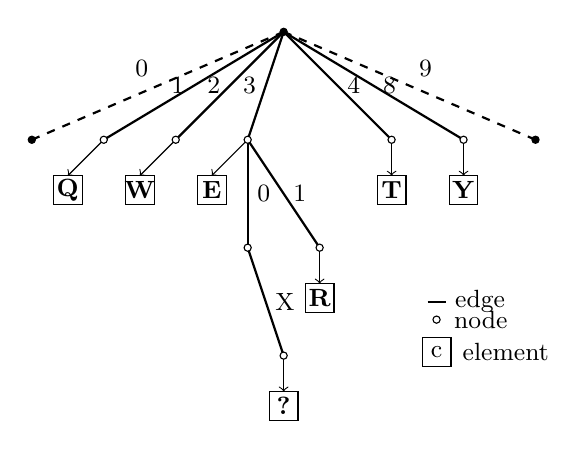
\begin{tikzpicture}[scale=1.3]

\newcommand\Y{-30};
\newcommand\ADDY{-10};

  %% node to node
  \small
  \draw[dashed,thick] (0pt,0pt) -- node[anchor=south east]{0} (-70pt,-30pt);
  \draw[thick] (0pt,0pt) -- node[anchor=east]{1} (-50pt,-30pt); %% Q
  \draw[thick] (0pt,0pt) -- node[anchor=east]{2} (-30pt,-30pt); %% W
  \draw[thick] (0pt,0pt) -- node[anchor=east]{3} (-10pt,-30pt); %% E
  \draw[thick] (0pt,0pt) -- node[anchor=west]{4} ( 30pt,-30pt); %% T
  \draw[thick] (0pt,0pt) -- node[anchor=west]{8} ( 50pt,-30pt); %% Y
  \draw[dashed,thick] (0pt,0pt) -- node[anchor=south west]{9} ( 70pt,-30pt);

  \draw[thick] (-10pt,-30pt) -- node[anchor=west]{1} ( 10pt,-60pt); %% R
  \draw[thick] (-10pt,-30pt) -- node[anchor=west]{0} (-10pt,-60pt);
  \draw[thick] (-10pt,-60pt) -- node[anchor=west]{X} (  0pt,-90pt); %% ?


  %% node to element
  \draw[->] (-50pt,\Y pt) -- (-60pt, \ADDY +\Y pt);
  \draw[->] (-30pt,\Y pt) -- (-40pt, \ADDY +\Y pt);
  \draw[->] (-10pt,\Y pt) -- (-20pt, \ADDY +\Y pt);
  \draw[->] ( 30pt,\Y pt) -- ( 30pt, \ADDY +\Y pt);
  \draw[->] ( 50pt,\Y pt) -- ( 50pt, \ADDY +\Y pt);

  \draw[->] ( 10pt,2 * \Y pt) -- ( 10pt, \ADDY + 2 * \Y pt);
  \draw[->] (  0pt,3 * \Y pt) -- (  0pt, \ADDY + 3 * \Y pt);

  %% nodes
  \draw[fill=black] ( 0pt,  0pt) circle (1pt); 
  \draw[fill=black] (-70pt, -30pt) circle (1pt); 
  \draw[fill=white] (-50pt, -30pt) circle (1pt); %% Q
  \draw[fill=white] (-30pt, -30pt) circle (1pt); %% W
  \draw[fill=white] (-10pt, -30pt) circle (1pt); %% E
  \draw[fill=white] ( 30pt, -30pt) circle (1pt); %% T
  \draw[fill=white] ( 50pt, -30pt) circle (1pt); %% Y
  \draw[fill=black] ( 70pt, -30pt) circle (1pt);

  \draw[fill=white] (-10pt, 2 * \Y pt) circle (1pt); %% R
  \draw[fill=white] ( 10pt, 2 * \Y pt) circle (1pt); %% x
  \draw[fill=white] (  0pt, 3 * \Y pt) circle (1pt); %% ?

  %% elements
  \draw[fill=white](-60pt,-4 + \ADDY + \Y pt)
  node{\textbf{Q}} +(-4pt,-4pt) rectangle +(4pt,4pt) ; %% Q
  \draw[fill=white](-40pt,-4 + \ADDY + \Y pt)
  node{\textbf{W}} +(-4pt,-4pt) rectangle +(4pt,4pt) ; %% W
  \draw[fill=white](-20pt,-4 + \ADDY + \Y pt)
  node{\textbf{E}} +(-4pt,-4pt) rectangle +(4pt,4pt) ; %% E
  \draw[fill=white]( 30pt,-4 + \ADDY + \Y pt)
  node{\textbf{T}} +(-4pt,-4pt) rectangle +(4pt,4pt) ; %% T
  \draw[fill=white]( 50pt,-4 + \ADDY + \Y pt)
  node{\textbf{Y}} +(-4pt,-4pt) rectangle +(4pt,4pt) ; %% Y

  \draw[fill=white]( 10pt,-4 + \ADDY + 2 * \Y pt)
  node{\textbf{R}} +(-4pt,-4pt) rectangle +(4pt,4pt) ; %% R
  \draw[fill=white](  0pt,-4 + \ADDY + 3 * \Y pt)
  node{\textbf{?}} +(-4pt,-4pt) rectangle +(4pt,4pt) ; %% ?



  \draw[thick](40pt,-75pt) -- (45pt,-75pt) node[anchor=west]{edge};
  \draw(42.5pt,-80pt) circle (1pt) node[anchor=west]{\ node};
  \draw(42.5pt,-89pt) node{c} node[anchor=west]{\ \ element}
  +(-4pt,-4pt)rectangle+(4pt,4pt);

\end{tikzpicture}
}
  \hspace{20pt}
  \subfloat[Disambiguators operate when same paths have been allocated.]
  [\label{fig:disexample}The tree uses disambiguators to maintain an
  equivalent state, even in presence of concurrent insertions resulting
  in same paths. For simplicity sake, only the disambiguators of
  \texttt{E}, \texttt{R}, and \texttt{T} are displayed.]
  {\input{input/desexample.tex}}
  \caption{Examples of 10-ary trees containing the sequence of characters
    \texttt{QWERTY}.}
\end{figure*}


Figure~\ref{fig:treemodelexample} shows the underlying 10-ary tree representing
a sequence. Like in the previous scenario, the initial sequence is \texttt{QWTY}
with the respective paths $[1]$, $[2]$, $[4]$ and $[8]$. The insertion of the
character \texttt{E} between the pairs $\langle [2],\, \texttt{W}\rangle$ and
$\langle [4],\, \texttt{T}\rangle$ results in the following pair:
$\langle [3],\, \texttt{E} \rangle$. Then the insertion of Character \texttt{R}
needs to start a new level since there is no room at the first level of the tree
for a new path between \texttt{E} and \texttt{T}. The resulting path may be
$[3.1]$ if label $1$ is chosen for the element \texttt{R} at the second
level. This would increase the depth of the tree in case there is an insertion
between the elements \texttt{E} and \texttt{R}. The new path would be $[3.0.X]$
where $0<X<10$ (recall that we assume a 10-ary tree). The total order
$(\mathcal{P},\,<_\mathcal{P})$ allows retrieving the sequence \texttt{QWERTY}.

\subsection{Disambiguation of concurrent cases}
\label{subsec:disambiguation}

% Two collaborators concurrently performing an operation on their respective
% replica may get different results after the integration of both
% operations. Indeed,
The order among paths $(\mathcal{P},\,<_\mathcal{P})$ is a total order when a
single collaborator edits. However, it becomes a partial order when the editing
session involves several collaborators. For instance, two collaborators
inserting a character at a same position in the sequence and at a same time may
end up with the same path. In such case the order of characters is not strictly
defined and may break the convergence property. Disambiguators use globally
unique markers to provide a total order among elements even in presence of
concurrent insertions. These markers usually comprise unique site identifiers
along with Lamport clocks~\cite{lamport1978time}. Each pair of
$\langle element,\,path\rangle$ is associated with a disambiguator.

\begin{definition}[Disambiguator]
  A disambiguator is a marker chosen in a set $\mathcal{D}$ paired with a total
  order $(\mathcal{D},\, <_\mathcal{D})$.
\end{definition}

Let the set of identifiers $\mathcal{I}$ be the set of unique triples
$\mathcal{I}:\mathcal{P}\times \mathcal{A}\times \mathcal{D}$. The composition
of the partial order ($\mathcal{P}$, $<_{\mathcal{P}}$) and the total order of
disambiguators ($\mathcal{D}$, $<_{\mathcal{D}}$) orders the elements of the
sequence identically at any replica.

\begin{definition}[Variable-size identifier]
  A variable-size identifier is a triple $\langle p,\, \alpha,\, d \rangle$
  chosen in $\mathcal{I}$ where $p$ is a path chosen in $\mathcal{P}$, $\alpha$
  is an element chosen in an alphabet $\mathcal{A}$, and $d$ is a disambiguator
  chosen in $\mathcal{D}$. The set $\mathcal{I}$ is paired with a dense total
  order $(\mathcal{I},\,<_\mathcal{I})$.
\end{definition}

Figure~\ref{fig:disexample} depicts a tree containing 6 elements with only 5
distinct paths. First, Collaborator $c_1$ inserts \texttt{QW}.  Then, the
collaborators $c_1$ and $c_2$ concurrently insert respectively \texttt{E} and
\texttt{T} which happens to generate an identical path: [$3$]. To solve the
order ambiguity, the disambiguator $\langle c_1,\, 3\rangle$ is associated with
\texttt{E}; the disambiguator $\langle c_2,\, 1\rangle$ is associated with
\texttt{T}. Retrieving the order of elements simply consists in comparing at
each level the paths, then the site identifiers, then the clocks. In this
example, \texttt{E} precedes \texttt{T} because $c_1 < c_2$. Then, Collaborator
$c_1$ inserts \texttt{Y} at the end of the sequence. Finally, she inserts
\texttt{R} between \texttt{E} and \texttt{T}. Since \texttt{E} and \texttt{T}
have an identical path, there is not enough room for new insertions at this
level. The allocation function chooses a path [$3.X$] where $0<X<10$. By copying
the disambiguator of \texttt{E} at the first level, it ensures that the new
identifier will follow the character \texttt{E} and precede the character
\texttt{T}.  Collaborators cannot influence the final position of the character
in the sequence using disambiguators, for disambiguators are automatically
computed without concerns about positions. The sequence of the example could
have ended in \texttt{QWTREY} and it would have needed a correction. It is worth
noting that the space complexity of disambiguators is upper-bounded by their
respective path. Therefore, we focus on paths in the rest of the paper.

\subsection{Choosing the smallest path}
\label{subsec:choosing}

The most critical part of sequences with variable-size identifiers consists in
creating the paths. The function that allocates the identifers must provide the
smallest possible paths without impairing future
allocations.

Algorithm~\ref{algo:crdtabstract} shows the general outlines of these
sequences. It divides the operations -- insert and delete -- into the local and
remote parts of the optimistic replication scheme. We can see that the core of
the algorithm and associated complexity lies in the local part of the insert
operation where it generates a path (cf. Line~\ref{line:allocpath}) and a
disambiguator (cf. Line~\ref{line:allocdes}). The function \textsc{convert2Path}
gets rid of the disambiguators of the identifiers in argument to keep paths
only. Without evidence of concurrency, it simply returns the paths contained in
the identifiers. Otherwise, it translates the identifiers into paths that
maintain the order following the order of paths
($\mathcal{P},\, <_{\mathcal{P}}$). For instance in Figure~\ref{fig:disexample},
the result of \textsc{convert2Path} with the identifiers of the character
\texttt{E} and the character \texttt{T} is the pair
$\langle [3.0],\, [3.9]\rangle$. The function \textsc{allocPath} allocates a new
path between these bounds.  \textsc{allocDis} decorates the path in order to
guarantee that the new identifier -- as the composition of a path, an element,
and a disambiguator -- consistently fall between the adjacent identifiers that
served to create it following the order of identifiers
($\mathcal{I}, \, <_\mathcal{I}$).

\begin{algorithm}[h]
  \input{input/crdtabstractalgo.tex}
  \caption{\label{algo:crdtabstract}General outlines of a sequence with
    variable-size identifiers.}
\end{algorithm}

The function \textsc{allocPath} chooses a path in the tree between two other paths
$p$ and $q$ where $p$ precedes $q$: $p<_{\mathcal{P}}q$. The new path $n$ must
fall between $p$ and $q$: $p<_\mathcal{P}n<_\mathcal{P}q$.
% However, the number of paths between two paths is infinite, for the order is
% dense, and so is the number of \textsc{allocPath} strategies. Nevertheless,
The function \textsc{allocPath} should choose the smallest available path among all
the possible paths for performance sake.
% This observation reduces considerably the number of possible allocation
% strategies.

\begin{figure*}
  \centering
  \subfloat[Optimal case.]
  [\label{fig:allocpathexampleA} Optimal case.]
  {\input{input/allocpathexampleA.tex}}
  \hspace{50pt}
  \subfloat[Worst case.]
  [\label{fig:allocpathexampleB} Worst case.]
  {\input{input/allocpathexampleB.tex}}
  \caption{\label{fig:allocpathexample} Two trees filled with the resulting
    identifiers of two different permutations resulting in an identical sequence
    \texttt{QWERTY}. The function \textsc{allocPath} allocates the leftmost
    branch in the tree. All paths of the optimal case have a length of 1 while
    the tree of the worst case grows up to a depth of 6.}
\end{figure*}

As illustrated in Figure~\ref{fig:allocpathexample}, the allocation of paths
without an \emph{a priori} knowledge of the final sequence is a non-trivial
problem.  Suppose that \textsc{allocPath} allocates the leftmost branch
available at the lowest depth possible. Suppose two insertion orders resulting
in an identical sequence of characters \texttt{QWERTY}.  In the first case,
\texttt{Q} is inserted first at position 0, followed by \texttt{W} at position 1
(after \texttt{Q}) then \texttt{E} is inserted at position 3 (after \texttt{W}),
etc.  In the second case, \texttt{Y} is inserted first at position 0 as the
sequence is initially empty. Then \texttt{T} is inserted. However as the final
intended word is \texttt{QWERTY}, \texttt{T} has to be inserted at a position
before \texttt{Y} that represents the current state of the sequence. \texttt{T}
is thus inserted at position 0 shifting \texttt{Y} to position 1, etc.


\begin{itemize}[noitemsep, leftmargin=*]
\item Figure~\ref{fig:allocpathexampleA}: In this case, the insertion order
  exactly follows the expectations of the allocation function. The depth of the
  tree never grows. The execution of operations remain efficient.

\item Figure~\ref{fig:allocpathexampleB}: In this case, the insertion order goes
  against the expectations of the allocation function. The depth of the tree
  increase at each insertion. Indeed, as an element gets the smallest value at
  its level, there is no room for a new element at the same level, hence the
  creation of a new level. The depth of the tree grows very fast decreasing the
  efficiency of operations.
\end{itemize}

This example shows how the insertion order impacts the length of the allocated
paths. Unfortunately, the insertion order cannot be predicted, nor the size of
the final sequence. Prior work on sequences often made the assumption of a
left-to-right editing due to observations made on
corpora~\cite{preguica2009commutative, weiss2009logoot}. However, there exist
human edited documents that do not correspond to this kind of
editing~\cite{nedelec2013lseq}.
%% Indeed, the editing depends on the type of the document and to the activity
%% for example when correcting a document the editing in mainly random as the
%% insertions and deletions corresponds to errors distributed in the document.
Hence the need of an allocation function which provides identifiers with a
sublinear space complexity compared to the number of insertions whatever is the
editing sequence. Such allocation function would avoid the need for consensus
algorithm~\cite{mostefaoui2015signature} and would make CRDT-based editors a
practicable alternative to the current mainstream editors.
 
%%% Local Variables:
%%% mode: latex
%%% TeX-master: "../paper"
%%% End:
